% Created 2024-10-16 śro 21:35
% Intended LaTeX compiler: pdflatex
\documentclass[../main.tex]{subfiles}
\usepackage[utf8]{inputenc}
\usepackage[T1]{fontenc}
\usepackage{graphicx}
\usepackage{longtable}
\usepackage{wrapfig}
\usepackage{rotating}
\usepackage[normalem]{ulem}
\usepackage{amsmath}
\usepackage{amssymb}
\usepackage{capt-of}
\usepackage{hyperref}
\usepackage[polish]{babel}
\usepackage[a4paper, margin=3cm]{geometry}
\usepackage{float}
\graphicspath{{../}}
\author{Wojciech Paderewski}
\date{\today}
\title{Koncepcja ukladu}
\hypersetup{
 pdfauthor={Wojciech Paderewski},
 pdftitle={Koncepcja ukladu},
 pdfkeywords={},
 pdfsubject={},
 pdflang={Polish}}
\begin{document}

\subsection{Złącze DC-Plug}
\subsubsection{Dlaczego złącze DC-Plug?}
Złącze DC jest złączem, które jest powszechnie stosowane w zasilaczach, co czyni je uniwersalnym rozwiązaniem, odpowiednim do tej aplikacji.
Wybrano złącze o jak najmniejszych rozmiarach, by zegar był jak najcieńszy. Złącze to zostało wybrane również ze względu na to, że łatwo znaleźć zasilacz 12V z takim złączem.

\subsubsection{Opis podłączenia}
Do złącza dołączono 3 kondensatory filtrujące, które mają za zadanie zminimalizować zakłócenia zasilania. 2 kondensatory o 
pojemności 100uF w celu zminimalizowania zakłóceń niskich częstotliwości, oraz 1 kondensator o pojemności 100nF w celu zminimalizowania zakłóceń wysokich częstotliwości.
\\\\
kondensatory 100uF są kondensatorami tantalowymi, a kondensator 100nF jest kondensatorem ceramicznym. Wykorzystano te rodzaje kondensatorów, 
ponieważ są to kondensatory o długiej żywotności, a także są to kondensatory o małych rozmiarach w przeciwieństwie do kondensatorów elektrolitycznych.

\subsubsection{Zabezpieczenia ESD}

W celu zabezpieczenia linii przed przepięciami, wykorzystano diodę TVS firmy Wurth Elektronik o symbolu 824045812. Dioda ta jest diodą TVS o napięciu przebicia 13.3V,
oraz napięciu stabilizacji 15V. Dioda musi mieć jak najmniejsze napięcie przebicia, by skok napięcia nie uszkodził rejestrów przesuwnych HV, które są wrażliwe na napięcia powyżej 13.2V.
\\\\
Dioda ta została wybrana gdyż nie udało się znaleźć diody TVS o napięciu stabilizacji 13V. Transil ma również dużą pojemność, co powoduje, że nie jest ona zalecana do 
zastosowań z wysokimi częstotliwościami, jednak w tym przypadku nie jest to problemem, gdyż jest to tylko złącze zasilania o stałym napięciu.

\subsubsection{Schemat}
\begin{figure}[H]
    \centering
    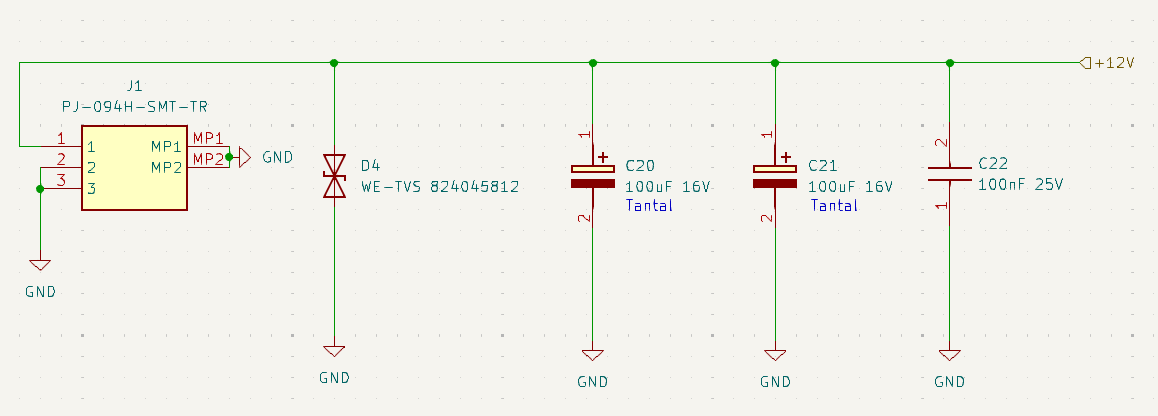
\includegraphics[width=0.8\textwidth]{DcPlug_schemat.png}
    \caption{Schemat złącza DC-Plug}
\end{figure}

\end{document}
